\documentclass[11pt]{article}
\usepackage[margin=.8in]{geometry}
\usepackage{amsmath,amssymb,graphicx,hyperref}
\setlength{\parindent}{0pt}\setlength{\parskip}{6pt}
\begin{document}
\begin{center}{\Large Actual growing point constraints produce an integral residual}\\27 November 2026 --- unsigned local Lean component evidence\end{center}
Over a field \(K\), retain an actual short Weierstrass curve, nonzero two,
and nonsingular points \(P_i=(x_i,y_i)\) with nonzero ordinates.
Choose \(d\ge0\), levels \(n_i\ge0\), and \(\sum_i n_i<2d+1\).
The actual coefficient space has \(d+1\) coefficients for \(A\) and \(d\) for \(B\).
Lean constructs a nonzero coordinate function \(h=A+BY\), with
\(\deg\operatorname{Norm}(h)\le2d+1\).
For injective coordinate pairs, it constructs an integral ideal \(J\) and derives
\[
 \langle h\rangle=\left(\prod_i I_{P_i}^{n_i}\right)J,
 \qquad \sum_i n_i+\dim_K(R/J)\le2d+1.
\]
The successful function, branch roots, kernel and residual are derived, not
supplied as favorable witnesses (PCC-20261127-379167) [pcc:unverified].
\begin{center}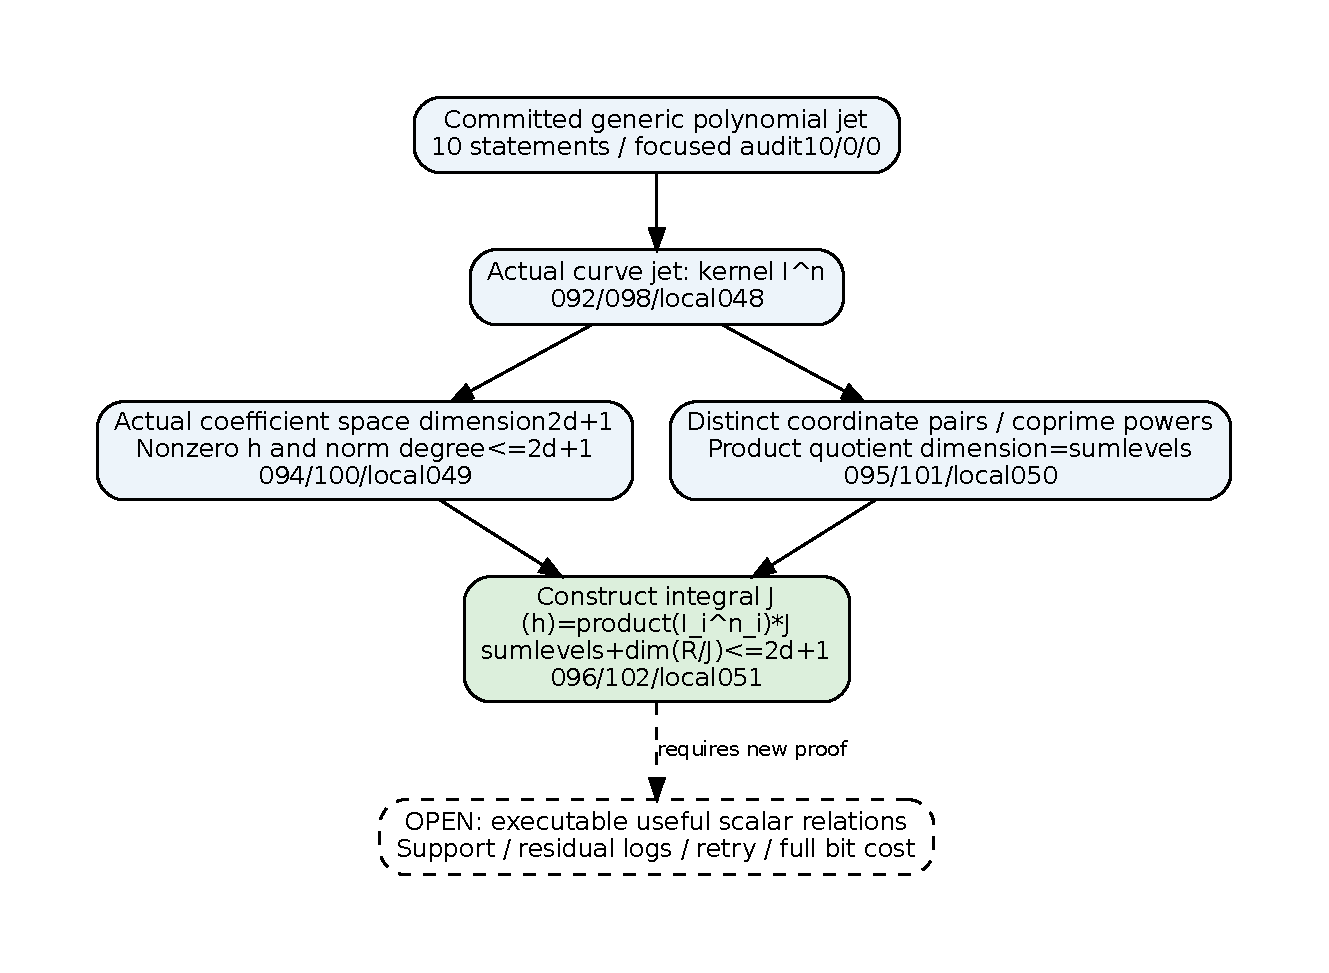
\includegraphics[width=.97\linewidth,height=4.5in,keepaspectratio]{growing-residual-dependencies-001.pdf}\end{center}
The dashed step remains a separate obligation. A small residual degree does
not supply a known logarithm or an efficient useful relation finder.
\newpage
\begin{center}{\Large Construction, checks and remaining obligations}\end{center}
\textbf{Local-to-global construction.}
The committed generic jet algebra is \(K[T]/(T^n)\), including \(n=0\).
The actual curve-to-jet map is surjective; its kernel is derived to be
\(I_P^n\), by ideal annihilation and the two actual quotient dimensions.
The actual coefficient map is injective. Its dimension is \(2d+1\), whereas
the actual family of jet targets has dimension \(\sum_i n_i\).
Strict inequality yields a nonzero actual constrained function [pcc:unverified].

Explicit generator differences prove coprimeness for distinct coordinate
pairs, including equal abscissas with different ordinates. Coprime powers
identify the actual product with the intersection; CRT gives quotient
dimension \(\sum_i n_i\). Actual point fractional units construct integral
\(J\). The previously committed generic invertible-ideal codimension law
and the actual norm degree give the additive bound [pcc:unverified].

\textbf{Validation map.}
\begin{center}\begin{tabular}{llll}
Source/build&Receipt&Printed&New scope\\
090/096&047&224&actual jet map and surjectivity\\
092/098&048&232&exact point-power kernel\\
094/100&049&242&growing nonzero function\\
095/101&050&248&global product and CRT\\
096/102&051&252&integral residual and bound
\end{tabular}\end{center}
All accepted runs exit zero with zero warnings and standard printed
foundations. Final252 includes217 prior statements and35 new endpoints.
All348 final dependency bindings were checked. Claims
PCC-20261127-48b69f,230077,134586,e3c997,379167 are unsigned local data,
outside historical shared Transport53/57 audit/fresh [pcc:unverified].
Failed089/091/093 sources, raw outputs and exits remain preserved.
The generic owner module has ten audited statements and zero extra trusted
axioms; its focus build does not imply a whole-project fresh replay.

\textbf{Controls and limits.}
Zero levels, empty families and \(d=0\) belong to the theorem domains.
Repeated points are allowed in individual constraints; the product theorem
explicitly requires injective coordinate pairs. Noncomputable choice and
linear algebra establish existence. Executable branch and coefficient
construction, kernel costs, useful known-label support, residual splitting
and logarithms, density, retries and full expected bit cost remain open.
The original weighted W-jet and nonscalar-origin interface is separate.

\textbf{Sources checked.}
Public Mathlib power-series truncation, Polynomial.OfFn, ideal quotient CRT;
actual NormGroupBridge coprimeness, residue-field and finite-quotient
proofs; committed generic polynomial-jet, integral-residual and ideal
codimension modules. These are standard
interpolation/local-algebra methods, without a novelty claim. KB unavailable;
source fallback only. Protocol016 and continuation026 record the next action.
\end{document}
